\section{Lindhard Model} 

When a particle interacts within a material it has the potential to excite electron-hole pairs into the conduction band, yielding the question: For a particle of a given energy, how much energy is given to the electrons, and how much energy loss is due to atomic motion? In the dark matter community, the most widely accepted model to answer this question is the Lindhard model. The Lindhard model predicts the percentage, or yield, of electron-hole pairs created in an interaction. A particle traversing a material has a high probability of scattering in multiple ways, meaning that the crosssections for interacting with the electrons or the nuclei compete for the dominant interaction. The total interaction is described by the following: \cite{Lindhard_3}



\begin{equation}
k \epsilon^{1/2}\nu^{'}(\epsilon) = \int_{0}^{\epsilon^{2}} \frac{dt}{2t^{\frac{3}{2}}}f(t^{1/2})(\nu(\epsilon -\frac{t}{\epsilon}) - \nu(\epsilon)+\nu(\frac{t}{\epsilon}))
\end{equation}
\noindent
Where

\begin{equation}
\epsilon = E\frac{a}{2Z^2e^2}
\end{equation}
is dimensionless energy, $\nu$ is the energy loss due to atomic motion, and $t$ is a variable representing the solid angle for a scatter at a given energy. Solving this equation for a non-screening potential gives an analytical form for the energy loss due to atomic motion:\cite{sorensen_atomic_2015} 

\begin{equation}
\nu(\epsilon) = \frac{\epsilon}{1+kg(\epsilon)}
\end{equation}
$g$ is a parameterization dependent upon the energy of , and $k$ is a constant that is determined by the material of interest. For Germanium k = 0.157. Since the quantity of interest is the amount of energy given to the electrons, $\nu(\epsilon)$ can be from the reduced energy to find the ionization yield for nuclear recoils. 


\begin{equation}
f_n = \frac{\epsilon - \nu(\epsilon)}{\epsilon} = \frac{kg(\epsilon)}{1+kg(\epsilon)}
\end{equation}




\begin{figure}[h]
\centering
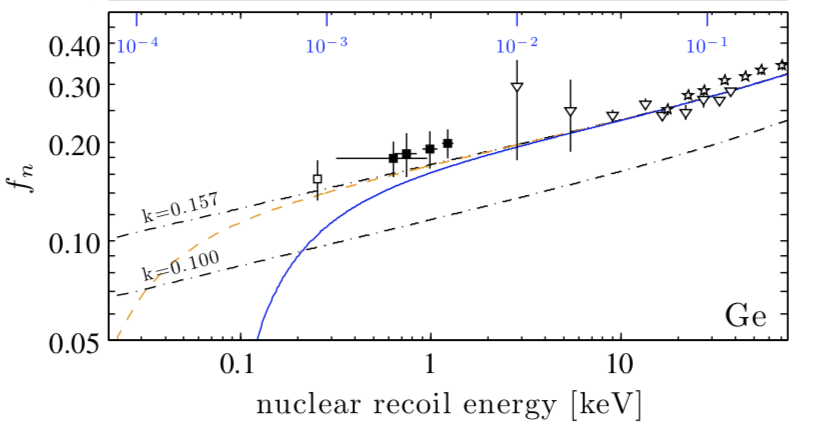
\includegraphics[scale=1]{Lindhard_Yield}
\caption{Lindhard Yield}
\end{figure}

\noindent
Figure 3.1 shows the Lindhard yield as a function of energy. The two dashed lines represent functions for two different materials. $k = 0.157$ is the line for Germanium and $k = 0.100$ is the line for silicon. The blue line represents a modification made to the Lindhard model that might be explored later. As shown, the model predicts energy given to the electronic system down to 0keV. \par





\section{Event Discrimination}

An atomic recoil results in the creation of electron-hole pairs and phonons. The distribution of energy from the recoil depends on the interacting particle and it's method of interaction, i.e whether the recoil is a nuclear recoil or an electronic recoil. By measuring the ionization yield mentioned in the previous section, it is possible to discriminate between events. \par

When the incoming particle interacts with the electronic system, the majority of the recoiling electrons energy goes into creating highly energetic electron-hole pairs. These electron-hole pairs lose their energy by the creation of phonons and other electron-hole pairs. The phonons created also have the ability to create further charge carriers and his process continues until there is not enough energy to create phonons or liberate more e-h pairs.\cite{phipps_ionization_2016} The result is an abundance of free e-h pairs that will be collected by their oppositely charged electrodes.\par


A recoiling neutron can create electron-hole pairs in the same manner as mentioned above, but can also lose some of it's energy by exciting other neutrons in the crystal lattice. A low energy recoiling nucleus has a lower probability of losing energy through the excitation of another nucleus or creating charge carriers. The excited nucleus will then lose all of its energy through the liberation of phonons. In the CDMSlite experiment, these phonons are what is measured. The phonon signal is measured through transition edge sensors, which are superconducting tungsten-aluminum sensors that readout signal by taking advantage of quasiparticle trapping and electrothermal feedback.\cite{TES} This mechanism consequently reduces the intermediate ionization signal, as it takes more energy from a nuclear recoil to liberate the same amount of charge carriers as an electron recoil.\cite{Transport} \par

When discriminating between electron and nuclear recoils, Luke-phonon production must be accounted for.[Carrier Thesis] Charge carriers that are accelerated across an electric potential will spontaneously emit phonons. Like the primary phonons created during the nuclear recoil, these phonons will be read by the TES and add to the overall measured signal. This combined signal must, therefore, be accounted for in the total measured energy signal. 

\begin{equation}
E_{measured} = E_{Recoil} + E_{Luke} = E_{Recoil}(1+\frac{q \Delta V}{\epsilon})
\end{equation}

As shown in figure 3.2, using the lindhard yield defined in equation 3.4 to compair the yield and the measured ionization energy can clearly show the discrimination between electron and nuclear recoils as the he different events seperate into distinct bands. The top band fitted in red is the electron recoil band and the bottom band fitted in blue is the nuclear recoil band. The red and blue fits are 2 $\sigma$ bands centered about the mean. \cite{Note_325} \par



 
\begin{figure}[h]
	\centering
	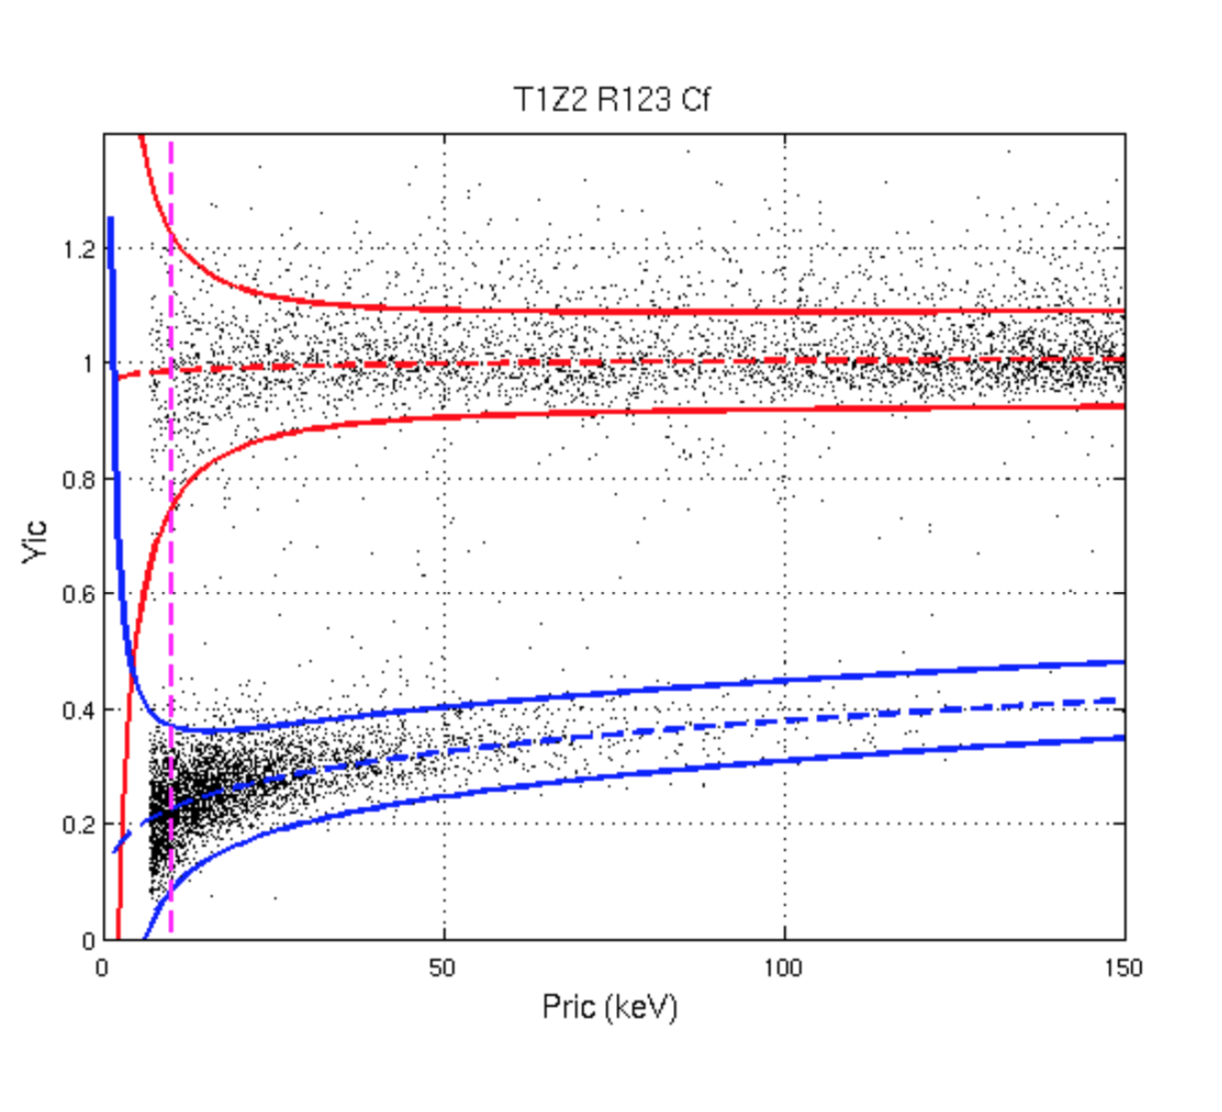
\includegraphics[scale=.55]{Yield_Bands}
	\caption{Atomic Recoil Bands }
\end{figure}

 

\section{"Fano Factor"}
The difference in width of the nuclear recoil bands is something that hasn't been looked at all that much. A possible explanation might be the need for a nuclear "fano factor." The quotes are needed as this is not the normal definition of a fano factor. A fano factor or constant of variation is defined as the measure of dispersion of a probability distribution, or the ratio of the variance to the mean, which is a purely statistical phenomenon. For example, if we assume a Poisson distribution, the Fano factor is equal to one as the variance is equal to the mean. In this case, the assumption is the "fano factor" might not be purely statistical and directly depend upon the energy of the recoiling nuclei. One approach is seen in \cite{Mei}, where they relate the variance in the energy bands to the normal definition of the fano factor, making it it energy dependent. 

\begin{equation}
\begin{gathered}
\sigma = \sqrt{NF}\\
\sigma =\sqrt{\frac{E_0}{\epsilon_i}}*\sqrt{\frac{E_x}{E_i}(\frac{\epsilon_i}{E_i}-1)}\
\end{gathered}
\end{equation} 
\noindent
Therefore 
\begin{equation}
\begin{gathered}
F = \sqrt{\frac{E_x}{E_i}(\frac{\epsilon_i}{E_i}-1)}
\end{gathered}
\end{equation} 
Here $E_x$ is the phonon energy, $E_i$ is the energy of the charge pairs, and $\epsilon_i$ is the energy required to create one election hole pair. The derivation of 3.10 is found in equation 5 in \cite{Mei}. Assuming Germanium with $\epsilon = 3.32 eV$, this method yields a fano factor of 0.16. This does lessen the difference in bandwidth but lacks experimental constraints \textbf{Talk Amy and Anthony more about this and need to add Dougherty info}\par
\noindent
Lindhard also makes a prediction for the width of the bands in terms of mean squared deviation $\Omega^2$, which is the variance with a reference point of 0.\cite{Lindhard_3}



\begin{figure}[h]
	\centering
	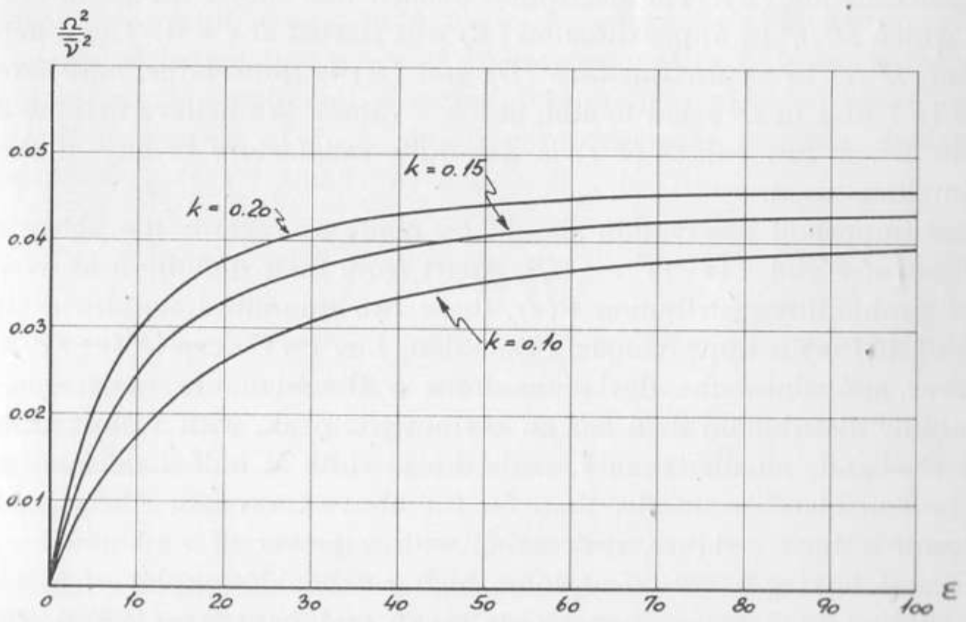
\includegraphics[scale=.65]{Lind_Var}
	\caption{Relative Mean Squared Deviation}
\end{figure}
\noindent
Figure 3.4 shows the relative mean squared variance for the energy loss due to atomic motion $\nu(\epsilon)$ for three different values of k. The meaning for $\Omega^2$ is straightforward if the probability of $\nu(\epsilon)$ is normally distributed, 

\begin{equation}
\begin{gathered}
P(\nu) = Ce^{\frac{-(\nu-\bar{\nu}^2)}{2*\Omega^2}}\\
\Omega^2 = <(\nu - \bar{\nu})^2>
\end{gathered}
\end{equation}
\noindent
and is useful if particles are collected individually. For many particles in a solid, it is useful to consider a Gaussian with mean $N\bar{\nu}$ and average square fluctuation of $N\Omega^2$.




